\documentclass[11pt,a4paper]{article}
\usepackage[utf8]{inputenc}
\usepackage[main=italian,provide=*]{babel}
\usepackage{amsmath,amssymb,amsthm}
\usepackage{mathtools}
\usepackage{geometry}
\geometry{margin=2.4cm}
\usepackage{graphicx}
\usepackage{enumitem}
\usepackage{booktabs}
\usepackage{array}
\usepackage{microtype}
\microtypesetup{expansion=false}
\usepackage{seqsplit}
\setlength{\emergencystretch}{3em}
\usepackage{xcolor}
\usepackage{tcolorbox}
\usepackage{hyperref}
\hypersetup{colorlinks=true,linkcolor=blue!50!black,urlcolor=blue!50!black}

\newtcolorbox{ideabox}[1][]{colback=blue!4,colframe=blue!45!black,
  fonttitle=\bfseries,title={#1},boxrule=0.6pt,left=4pt,right=4pt,top=3pt,bottom=3pt}
\newtcolorbox{warnbox}[1][]{colback=orange!5,colframe=orange!60!black,
  fonttitle=\bfseries,title={#1},boxrule=0.6pt,left=4pt,right=4pt,top=3pt,bottom=3pt}
\newtcolorbox{noveltybox}[1][]{colback=green!4,colframe=green!35!black,
  fonttitle=\bfseries,title={#1},boxrule=0.6pt,left=4pt,right=4pt,top=3pt,bottom=3pt}

\newtheorem{proposizione}{Proposizione}
\newtheorem{lemma}{Lemma}
\newtheorem{corollario}{Corollario}

\newcommand{\ket}[1]{\lvert #1\rangle}
\newcommand{\bra}[1]{\langle #1\rvert}

\title{Il circuito per le correlazioni dinamiche del trimero a catena aperta\\
\large Dallo stato fondamentale alla misura, passo per passo --- mirror per la topologia a due legami}
\author{Note di lavoro --- tesi triennale in Fisica (UniPR)\\
Relatore: Prof.\ Alessandro Chiesa}
\date{\today}

\begin{document}
\maketitle

\begin{abstract}
\noindent
Spiegazione completa e autocontenuta del circuito quantistico che misura la funzione di
correlazione dinamica $C_{ij}^{\alpha\beta}(t)=\langle\psi_0|\sigma_i^\alpha(t)\,
\sigma_j^\beta(0)|\psi_0\rangle$ sul trimero a catena aperta di spin-1/2, con interazione di
Dzyaloshinskii--Moriya. Questo documento è il \emph{mirror} per la topologia a due legami di
\texttt{circuito\_correlazioni\_trimero\_anello\_spiegato.tex}: stessa struttura, stesso livello di
dettaglio, adattato dove i due bond (invece di tre) introducono differenze reali. Una differenza è
\textbf{qualitativa e opposta}, non solo quantitativa: il sito fisso della simmetria residua
($P_{13}$, non $U_\text{anello}$) qui \textbf{non} protegge alcun correlatore dall'annullarsi,
mentre nell'anello il sito fisso (3) dava quattro zeri rigorosi per ogni $t$ -- il documento lo
evidenzia con una figura di \emph{contrasto}, non con l'ennesima conferma dello stesso fenomeno.
Il blocco $U(t)$ mantiene comunque una struttura Trotter a due livelli, per lo stesso motivo
algebrico dell'anello (bond che condividono un qubit), solo con due bond invece di tre.
\end{abstract}

\tableofcontents

% =====================================================================
\section{Il punto di partenza e il problema}
% =====================================================================

\subsection{Cosa abbiamo già}

Al punto di lavoro VQE-DM ($J=1$, $b=b_c=3.0$, $D=0.15$ --- vedi
\texttt{\seqsplit{simmetrie\_correlatori\_trimero\_catena.tex}} per la scelta e la sua verifica)
l'Hamiltoniana è
\begin{align}
H ={}& \underbrace{J\big(\boldsymbol\sigma_1\!\cdot\!\boldsymbol\sigma_2
     + \boldsymbol\sigma_2\!\cdot\!\boldsymbol\sigma_3\big)}_{\text{scambio, }H_{ex}}
     + \underbrace{b\,(Z_1+Z_2+Z_3)}_{\text{Zeeman}} \notag\\
     &+ \underbrace{D\,(T_{12}-T_{23})}_{\text{Dzyaloshinskii--Moriya}},
     \qquad T_{ij}\equiv X_iZ_j-Z_iX_j,
\label{eq:H}
\end{align}
in convenzione Pauli diretta, su tre qubit (nessun mapping fermionico), solo due legami fisici
($(1,2)$ e $(2,3)$, nessun $(3,1)$). Convenzione sito$\leftrightarrow$qubit (identica in tutto il
progetto trimero): $\text{sito }1\to q_2$, $\text{sito }2\to q_1$, $\text{sito }3\to q_0$.

\begin{warnbox}[Lezione imparata dal dimero e dall'anello, applicata qui]
Una mappa sito$\leftrightarrow$qubit invertita è stata un bug reale nel circuito del dimero,
mascherato dalla simmetria sui primi correlatori testati. Qui la mappa è dichiarata una volta per
tutte (\texttt{trotter\_trimero\_catena.py}) e la validazione (Sez.~\ref{sec:validazione}) include
esplicitamente un test con \textbf{stato iniziale asimmetrico} sotto $P_{13}$: con il ground state
(che \emph{è} autostato di $P_{13}$) un mapping invertito sarebbe stato invisibile a qualunque
altro test di questa fase.
\end{warnbox}

Il VQE con DM (ansatz \texttt{W-2qC.K2}, $10$ parametri, fedeltà $\mathcal F=1$ a precisione
macchina su $15$ restart, vedi \texttt{vqe\_w2qC\_k2\_trimero\_catena.py}) ha prodotto lo stato
fondamentale, non degenere:
\begin{equation}
E_0=-7.369247,\qquad E_1-E_0=0.734742.
\end{equation}
Come per anello e dimero, questo stato compare nel circuito come blocco di \emph{state
preparation}. Il modulo \texttt{circuito\_correlazioni\_trimero\_catena.py} supporta due varianti,
selezionabili con l'argomento \texttt{ansatz\_params} di \texttt{build\_correlator\_circuit}: la
preparazione esatta delle ampiezze (\texttt{QuantumCircuit.prepare\_state}) e la preparazione via
il \emph{circuito VQE reale} \texttt{W-2qC.K2}. Il confronto sistematico delle 81 combinazioni fra
le due varianti (\texttt{validate\_vqe\_circuito\_correlazioni\_catena.py}) dà un errore medio
$1.9\times10^{-8}$ e massimo $5.9\times10^{-8}$ --- dell'ordine di $\sqrt{1-\mathcal F}$, come
atteso.

\subsection{Cosa vogliamo calcolare}

L'oggetto di interesse resta
\begin{equation}
\boxed{\;C_{ij}^{\alpha\beta}(t) \;=\; \langle\psi_0|\;\sigma_i^\alpha(t)\;\sigma_j^\beta(0)\;|\psi_0\rangle\;}
\label{eq:Cdef}
\end{equation}
con $i,j\in\{1,2,3\}$, $\alpha,\beta\in\{x,y,z\}$: $81$ combinazioni, \textbf{come nell'anello},
nonostante i due bond invece di tre. Il conteggio $3\times3\times3\times3$ dipende dal numero di
\emph{siti} del sistema, non dai legami dell'Hamiltoniana: $C_{13}^{\alpha\beta}(t)$ resta un
osservabile ben definito e generalmente non nullo anche se il legame $(1,3)$ non esiste, perché
$U(t)$ propaga comunque la correlazione tramite il sito $2$ intermedio (verificato numericamente,
vedi \texttt{simmetrie\_correlatori\_trimero\_catena.tex}, Sez.~1). Non si ripete qui la
discussione fisica del significato di $C_{ij}^{\alpha\beta}$ (risposta dinamica, si veda
\texttt{circuito\_correlatori\_spiegato.tex}, Sez.~1.2).

\subsection{Perché non si può misurare direttamente}

Argomento indipendente dalla topologia (identico a dimero e anello): per $t\neq0$,
$\sigma_i^\alpha(t)\sigma_j^\beta(0)$ non è hermitiano perché
$[\sigma_i^\alpha(t)\sigma_j^\beta(0)]^\dagger=\sigma_j^\beta(0)\sigma_i^\alpha(t)$, che coincide
con l'operatore di partenza solo se i due fattori commutano --- falso in generale per $t\neq0$.
$C_{ij}^{\alpha\beta}(t)$ è quindi in generale complesso, non misurabile direttamente.

\begin{ideabox}[L'idea centrale, invariata]
Non si misura il correlatore: si costruisce uno stato in cui il correlatore compare come
\emph{ampiezza di interferenza} fra due cammini, letta su un qubit ausiliario (l'ancilla). Identico
a dimero e anello: cambia solo la dimensione del registro (qui $8$, come nell'anello), non la
logica.
\end{ideabox}

% =====================================================================
\section{Il caso interessante: quando lo zero \emph{non} c'è}
\label{sec:caso2}
% =====================================================================

Per il dimero e l'anello questa sezione mostra \emph{dove} compare uno zero strutturale. Per la
catena la domanda pedagogicamente utile è l'opposta: la catena \emph{ha} un sito fisso sotto la
sua simmetria residua, esattamente come l'anello -- perché allora non produce zeri?

La simmetria residua della catena è $P_{13}$ (riflessione siti $1,3$, sito $2$ fisso), derivata e
verificata in \texttt{simmetrie\_correlatori\_trimero\_catena.tex}:
\begin{equation}
P_{13}\,\sigma_i^\alpha\,P_{13}^{-1}=\lambda_\alpha\,\sigma_{\pi(i)}^\alpha,
\qquad\pi=(1\,3),\qquad\lambda_\alpha\equiv+1\ \ \forall\alpha.
\end{equation}
Applicato al sito fisso $i=2$: $C_{22}^{\alpha\beta}(t)=\lambda_\alpha\lambda_\beta\,
C_{22}^{\alpha\beta}(t)$, cioè $C_{22}^{\alpha\beta}(t)=C_{22}^{\alpha\beta}(t)$ --- tautologico,
\textbf{nessun vincolo}, perché $\lambda_\alpha\lambda_\beta=+1$ sempre.

\begin{corollario}[già dimostrato in \texttt{simmetrie\_correlatori\_trimero\_catena.tex}, qui richiamato]
Nessuna combinazione $C_{22}^{\alpha\beta}(t)$ è forzata a zero per alcun $t>0$.
\end{corollario}

La Fig.~\ref{fig:sito2} mostra $C_{22}^{xz}(t)$ su un intervallo continuo: a $t=0$ è esattamente
zero (ma per un motivo \emph{diverso} --- il Cor.\ zero-t0-same, $\langle\sigma_2^y\rangle=0$ per
stato reale, non una conseguenza di $P_{13}$), mentre per $t>0$ cresce fino a $\sim0.54$: nessuno
zero rigoroso.

\begin{figure}[htbp]
\centering
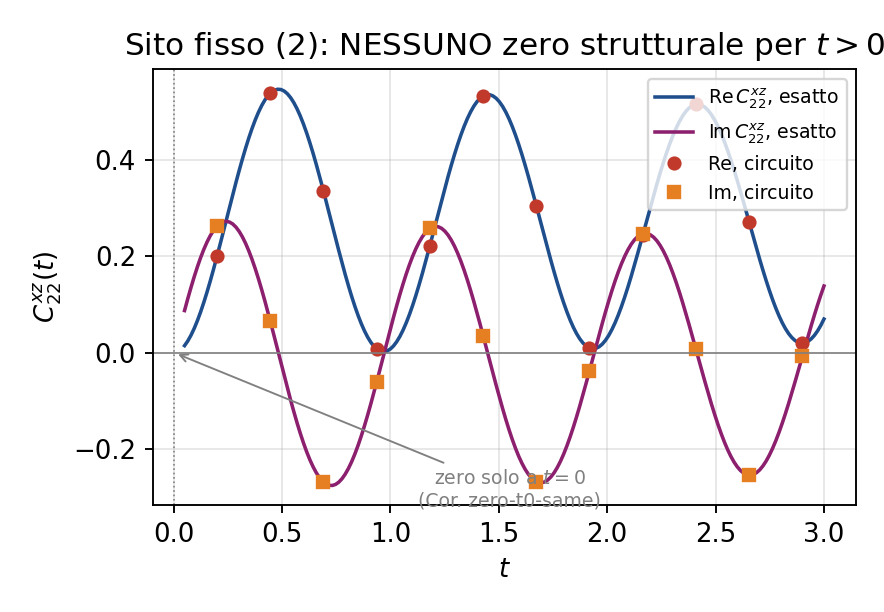
\includegraphics[width=0.62\textwidth]{fig_sito2_non_zero_trimero_catena.png}
\caption{$C_{22}^{xz}(t)$: il calcolo classico esatto (linee) confrontato con il circuito
quantistico ($N{=}200$, punti). Zero \textbf{solo} a $t=0$ (Cor.\ zero-t0-same, un argomento di
time-reversal, non di $P_{13}$); per $t>0$ il correlatore cresce fino a $\sim0.54$ ---
\textbf{contrasto diretto} con l'anello, dove il correlatore analogo sul sito fisso
($C_{33}^{xz}$) è identicamente zero per \emph{ogni} $t$.}
\label{fig:sito2}
\end{figure}

\begin{noveltybox}[Perché la catena non eredita lo zero dell'anello]
La differenza è nel segno: l'anello richiede $U_\text{anello}=\mathrm{SWAP}_{12}\cdot
(R_z(\pi))^{\otimes3}$, una vera rotazione oltre allo scambio che introduce $\eta_x=\eta_y=-1$;
la catena richiede solo $P_{13}=\mathrm{SWAP}$ puro, $\lambda_\alpha=+1$ sempre. Non è una
differenza di dettaglio tecnico: riflette l'assenza di frustrazione nella catena (nessun ciclo di
legami), verificata algebricamente (Sez.~3, \texttt{simmetrie\_correlatori\_trimero\_catena.tex})
prima di essere qui illustrata su un correlatore concreto.
\end{noveltybox}

\subsection{Il qubit ausiliario e la sovrapposizione di cammini}

Identico a dimero e anello: si aggiunge un'ancilla $a$, $\mathcal H=\mathcal H_a\otimes\mathcal
H_R$ con $\mathcal H_R$ a tre qubit (dimensione $8$). Da $\ket0_a\ket{\psi_0}_R$, Hadamard
sull'ancilla:
\begin{equation}
\ket{\Phi_1}=\tfrac{1}{\sqrt2}\big(\ket0_a+\ket1_a\big)\otimes\ket{\psi_0}_R.
\end{equation}

\subsection{Gate controllati e anti-controllati}

Definizioni invariate:
\begin{equation}
\mathrm{C}\text{-}G = \ket0\!\bra0_a\otimes\mathbb I_R + \ket1\!\bra1_a\otimes G_R,
\qquad
\mathrm{C}_0\text{-}G = \ket0\!\bra0_a\otimes G_R + \ket1\!\bra1_a\otimes\mathbb I_R.
\end{equation}

% =====================================================================
\section{Costruzione del circuito, stato per stato}
% =====================================================================

Esempio concreto, ripreso nelle figure: $C_{11}^{yy}(t)$ ($W=\sigma_1^y$ al tempo $0$,
$V=\sigma_1^y$ al tempo $t$ --- un'autocorrelazione, scelta perché è quella usata per la
validazione continua di Sez.~\ref{sec:trotter}).

\paragraph{Stadio 0 --- preparazione.} $\ket{\Phi_0}=\ket0_a\ket{\psi_0}_R$.

\paragraph{Stadio 1 --- Hadamard sull'ancilla.}
$\ket{\Phi_1}=\tfrac1{\sqrt2}(\ket0_a\ket{\psi_0}+\ket1_a\ket{\psi_0})$.

\paragraph{Stadio 2 --- controlled-$W$.} $W=\sigma_1^y$ sul qubit $Q[1]=q_2$, controllo pieno
dall'ancilla: $\ket{\Phi_2}=\tfrac1{\sqrt2}(\ket0_a\ket{\psi_0}+\ket1_a\,W\ket{\psi_0})$.

\paragraph{Stadio 3 --- evoluzione $U(t)$, senza controllo.}
$\ket{\Phi_3}=\tfrac1{\sqrt2}(\ket0_a\,U(t)\ket{\psi_0}+\ket1_a\,U(t)W\ket{\psi_0})$.

\paragraph{Stadio 4 --- anti-controlled-$V$.} $V=\sigma_1^y$ sullo stesso qubit $Q[1]=q_2$:
\begin{equation}
\boxed{\;\ket{\Phi_4}=\frac1{\sqrt2}\Big(\ket0_a\,\underbrace{VU(t)\ket{\psi_0}}_{\ket A}
+\ket1_a\,\underbrace{U(t)W\ket{\psi_0}}_{\ket B}\Big).}
\label{eq:phi4}
\end{equation}

La Fig.~\ref{fig:circuito} mostra le due esecuzioni (Re/Im) per un correlatore cross-site,
$C_{12}^{yy}(t)$ ($W=\sigma_2^y$ sul qubit $Q[2]=q_1$, $V=\sigma_1^y$ sul qubit $Q[1]=q_2$),
con $U(t)$ come box opaco (struttura interna in Sez.~\ref{sec:trotter}).

\begin{figure}[htbp]
\centering
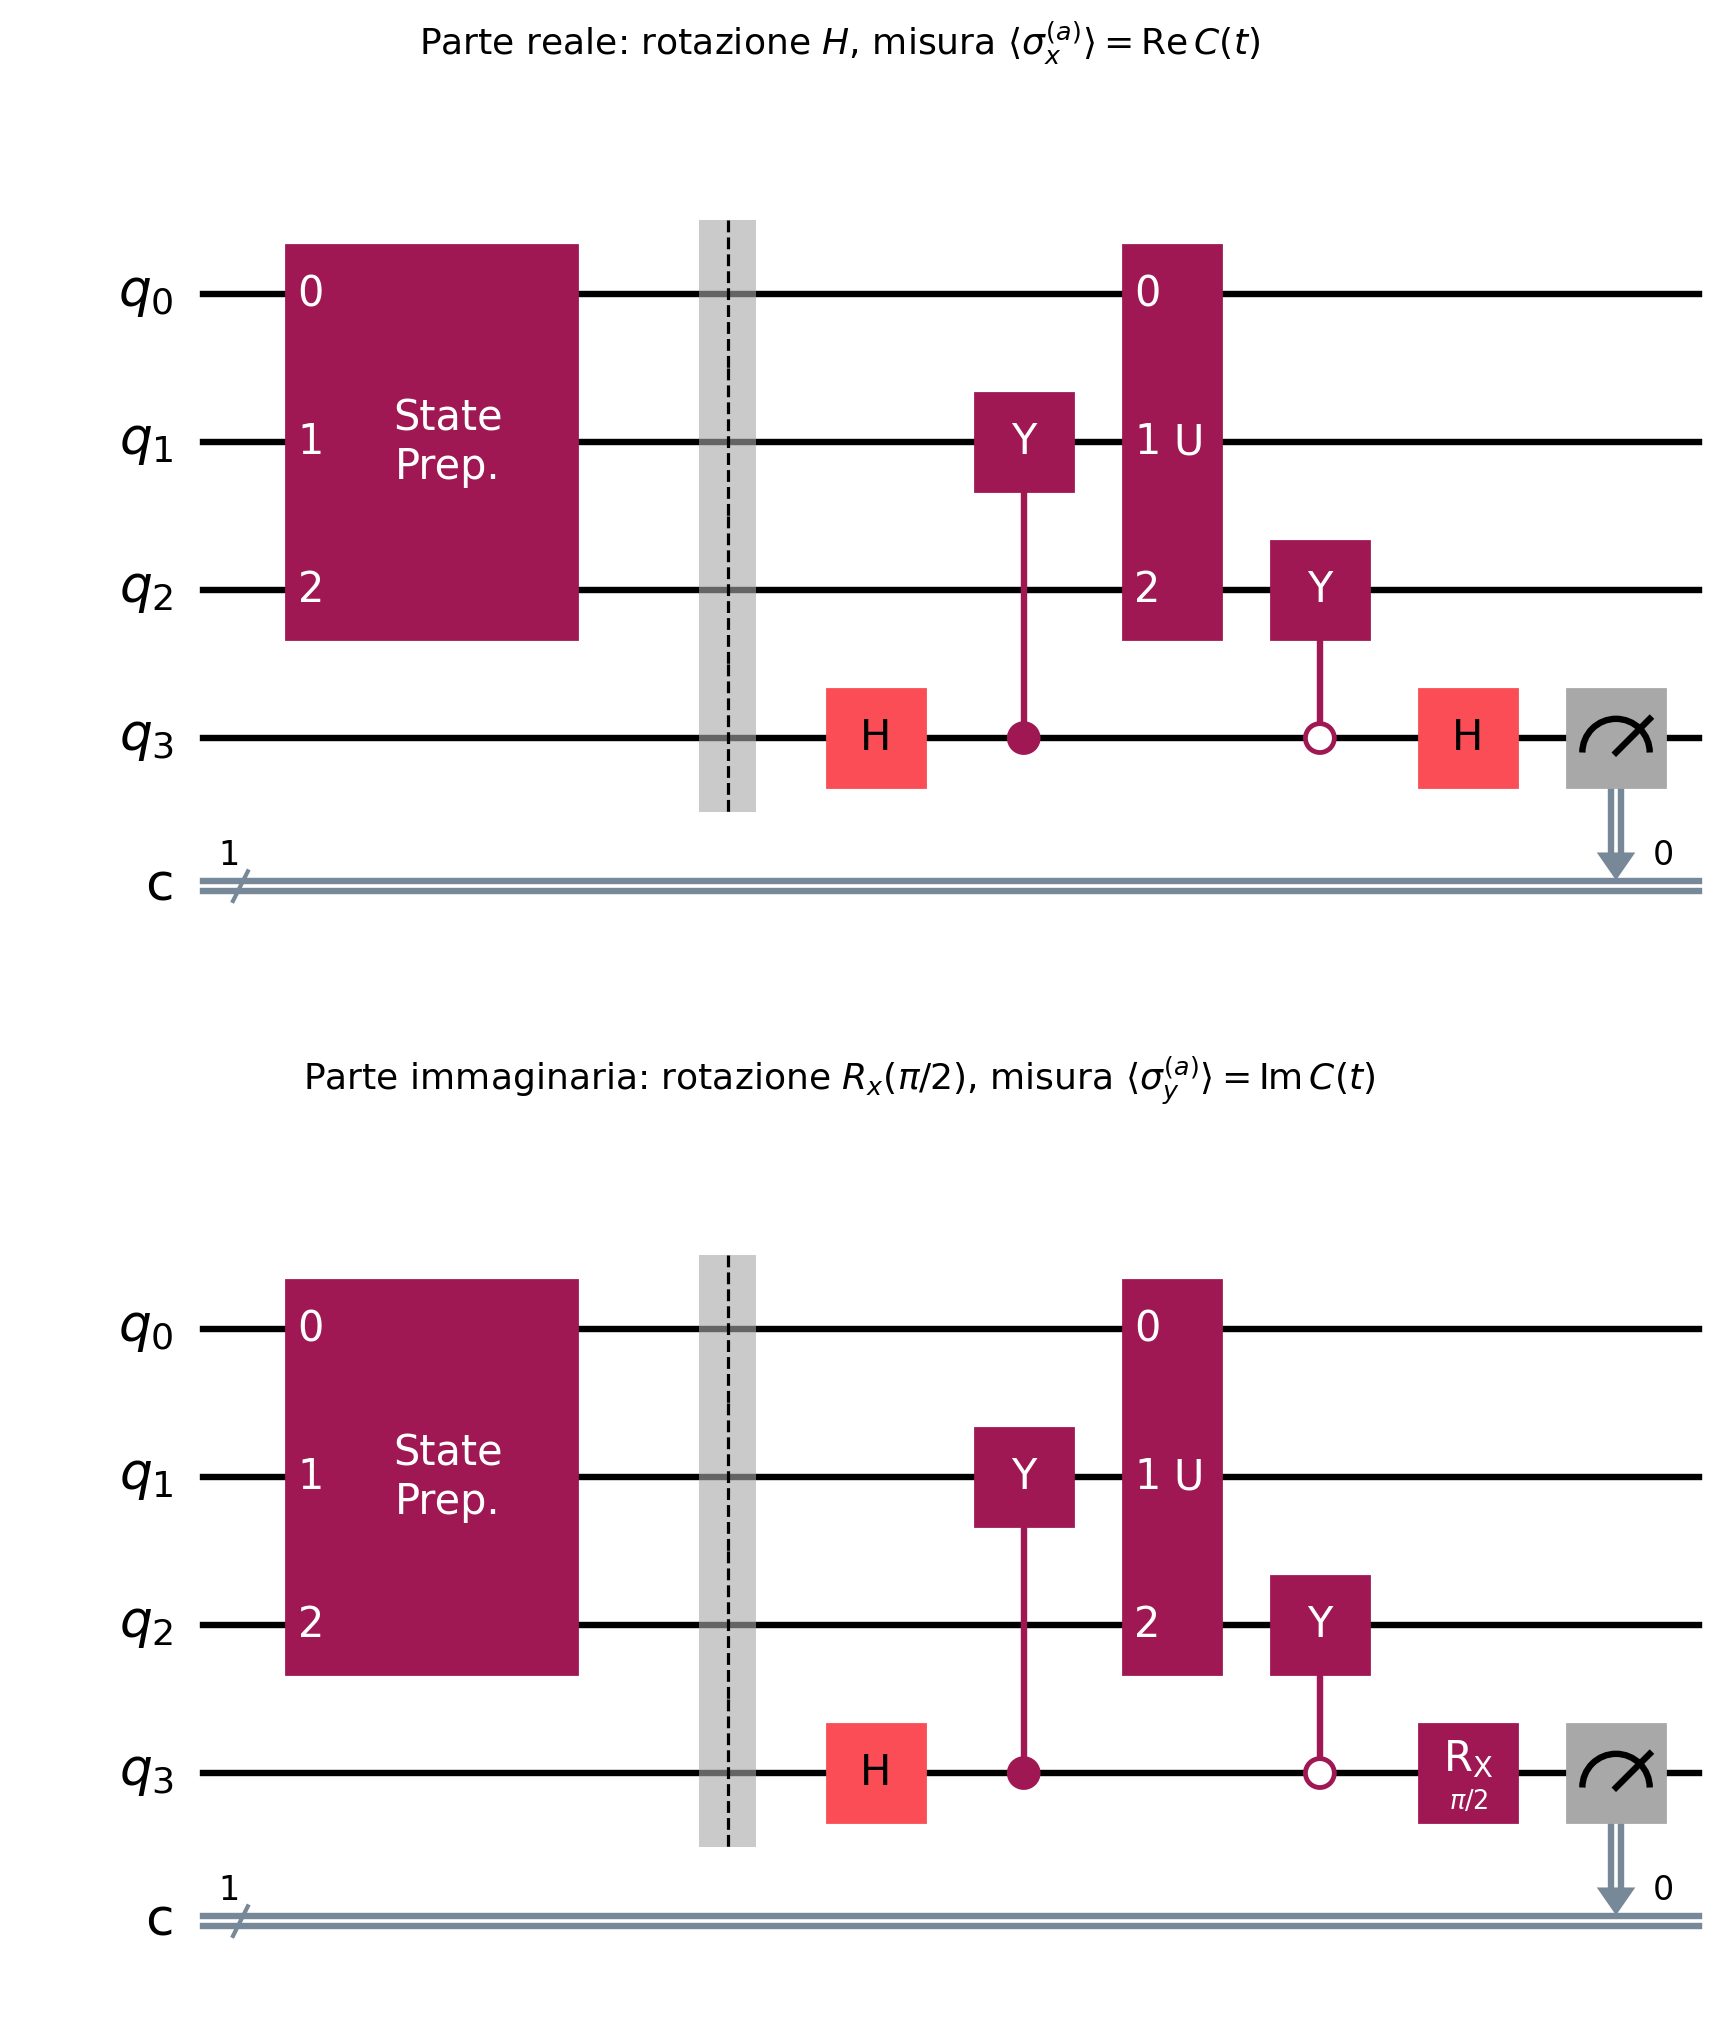
\includegraphics[width=0.72\textwidth]{fig_circuito_trimero_catena.png}
\caption{Le due esecuzioni del circuito per $C_{12}^{yy}(t)$: registro a 3 qubit ($q_0,q_1,q_2$)
più ancilla ($q_3$). Preparazione dello stato; Hadamard sull'ancilla; controlled-$Y$ su
$q_1=Q[2]$ (controllo pieno, $W=\sigma_2^y$); blocco $U(t)$ non controllato; anti-controlled-$Y$
su $q_2=Q[1]$ ($V=\sigma_1^y$). \emph{Sopra}: $H$ e misura
$\Rightarrow\langle\sigma_x^{(a)}\rangle=\mathrm{Re}\,C(t)$. \emph{Sotto}: $R_x(\pi/2)$ e misura
$\Rightarrow\langle\sigma_y^{(a)}\rangle=\mathrm{Im}\,C(t)$.}
\label{fig:circuito}
\end{figure}

% =====================================================================
\section{Perché funziona: la lettura dell'ancilla}
% =====================================================================

Indipendente dalla topologia (dimostrazione identica al dimero e all'anello, usa solo unitarietà
di $U(t)$ ed hermitianità di $V,W$):

\begin{proposizione}
Con $\ket A=VU(t)\ket{\psi_0}$, $\ket B=U(t)W\ket{\psi_0}$, $V,W$ hermitiani:
$\langle A|B\rangle=C_{ij}^{\alpha\beta}(t)$.
\end{proposizione}
\begin{proof}
$\langle A|B\rangle=(VU\ket{\psi_0})^\dagger(UW\ket{\psi_0})=\bra{\psi_0}U^\dagger V^\dagger U\,
W\ket{\psi_0}$, e $U^\dagger V^\dagger U=e^{iHt}Ve^{-iHt}=\sigma_i^\alpha(t)$.
\end{proof}

\begin{proposizione}
Nello stato \eqref{eq:phi4}: $\langle\sigma_x^{(a)}\rangle=\mathrm{Re}\,\langle A|B\rangle$,
$\langle\sigma_y^{(a)}\rangle=\mathrm{Im}\,\langle A|B\rangle$.
\end{proposizione}

Quindi il numero complesso non misurabile è scomposto in due osservabili hermitiane su un
singolo qubit ausiliario, indipendentemente da quanti legami ha $H$.

% =====================================================================
\section{Due punti delicati, verificati numericamente}
% =====================================================================

\subsection{Perché $U(t)$ non è controllato}

Se $U(t)$ fosse controllato, l'overlap finale conterrebbe $V^\dagger U$ invece di
$U^\dagger V^\dagger U$: non l'operatore di Heisenberg. Verifica numerica su $C_{11}^{yy}(t)$:

\begin{center}
\begin{tabular}{cccc}
\toprule
$t$ & valore esatto & $U$ non controllato & $U$ controllato \\
\midrule
$0.5$ & $-0.2668-0.1400i$ & $-0.2660-0.1388i$ & $\phantom{-}0.1561+0.2577i$ \\
$1.3$ & $+0.3243-0.4919i$ & $+0.3244-0.4922i$ & $-0.3965+0.4358i$ \\
\bottomrule
\end{tabular}
\end{center}
Stessa conclusione di dimero e anello: un errore che non produce un crash, va escluso per
costruzione.

\subsection{Controllo o anti-controllo su $V$?}

Con $V$ hermitiana (ogni Pauli), controllo pieno e anti-controllo sono equivalenti; si mantiene
l'anti-controllo per coerenza con la letteratura di riferimento.

% =====================================================================
\section{Il blocco $U(t)$: Trotter a due livelli, con due bond}
\label{sec:trotter}
% =====================================================================

\subsection{Perché un livello di Trotter non basta (anche con soli due bond)}

Come nell'anello, $H_0=b\sum_iZ_i+H_{ex}$ si fattorizza esattamente ($[S_z^{\rm tot},H_{ex}]=0$
bond per bond, verificato), ma $H_{ex}=J(\boldsymbol\sigma_1\!\cdot\!\boldsymbol\sigma_2+
\boldsymbol\sigma_2\!\cdot\!\boldsymbol\sigma_3)$ \textbf{non} è un blocco unico esponenziabile:
i due bond condividono il qubit $2$, e
$[\boldsymbol\sigma_1\!\cdot\!\boldsymbol\sigma_2,\boldsymbol\sigma_2\!\cdot\!\boldsymbol\sigma_3]
=-2i\chi\neq0$ (stessa chiralità di spin scalare $\chi$ dell'anello, identità verificata a residuo
$0.0$ esatto). Analogamente per $H_{DM}$, che genera un secondo operatore
$\Theta=X_1Y_2Z_3-Z_1Y_2X_3$, indipendente da $\chi$ (non assorbibile in una ridefinizione del
livello 1). Servono quindi due Trotter interni, uno per $H_{ex}$ e uno per $H_{DM}$, oltre al
Trotter esterno fra $H_0$ e $H_{DM}$:
\begin{equation}
e^{-iHt}\approx\Big(e^{-iH_{DM}\tau}\,e^{-i(b\sum Z_i)\tau}\,e^{-iH_{ex}\tau}\Big)^N,
\qquad
e^{-iH_{ex}\tau}\approx e^{-iJ\,\boldsymbol\sigma_2\cdot\boldsymbol\sigma_3\,\tau}\,
e^{-iJ\,\boldsymbol\sigma_1\cdot\boldsymbol\sigma_2\,\tau}.
\end{equation}

\begin{ideabox}[In una frase: due bond bastano per lo stesso fenomeno]
Non serve la chiusura ad anello per avere un secondo livello di Trotter: basta che due bond
qualsiasi condividano un qubit. La catena lo mostra con la struttura minima possibile (due bond),
la stessa identità algebrica dell'anello ($\chi$), un solo bond in comune invece di tre coppie.
\end{ideabox}

\begin{noveltybox}[Novità rispetto all'anello: l'alternanza dei bond]
Il segno del termine chirale di livello 1 dipende dall'ordine di applicazione dei bond
(verificato: $s=+1.000$ per $(1,2)\to(2,3)$, $s=-1.000$ per l'ordine inverso). Alternare l'ordine
a passi consecutivi (\texttt{alternate=True} in \texttt{trotter\_trimero\_catena.py}) cancella il
termine chirale al leading order, portando l'errore da $O(1/N^2)$ a $O(1/N^4)$ a $D=0$ (guadagno
$34\times$ misurato a $N=80$) --- ma il guadagno satura ed è addirittura \textbf{negativo} a $N$
piccolo quando $D\neq0$ (verificato: a $N=20$, fisso $9.7\times10^{-3}$ contro alternato
$1.3\times10^{-2}$). Non presente nel modulo Trotter dell'anello: è un affinamento specifico della
catena, non ancora usato di default (\texttt{alternate=False}) proprio per questa cautela.
\end{noveltybox}

\subsection{Convergenza al punto di lavoro delle correlazioni}

La Fig.~\ref{fig:trotter} mostra, per $C_{11}^{yy}(t{=}1.3)$, che l'errore scala come $1/N$
(rapporto fra errori successivi $\to2.0$ raddoppiando $N$), coerente con Trotter al 1° ordine; a
$N=200$ l'errore residuo è $\sim10^{-3}$.

\begin{warnbox}[Perché i punti non giacciono esattamente sulla retta tratteggiata]
La retta $1/N$ in figura è ancorata al primo punto ($N=10$), non è l'asintoto vero: un fit
indipendente $\text{errore}\approx a/N+b/N^2$ sui 6 punti dà $a=4.60\times10^{-2}$,
$b=-0.258$. Il segno negativo di $b$ significa che a $N$ piccolo il termine subleading
\emph{sottrae} dall'errore leading-order (a $N{=}10$ il puro $a/N$ varrebbe
$4.6\times10^{-3}$, più del doppio dell'errore osservato $2.1\times10^{-3}$): il punto usato
per ancorare la retta è ancora fuori dal regime asintotico. Il rapporto fra errori successivi
lo conferma: $1.10$--$1.55$ a $N$ basso, $\to1.92$ solo per $N=160\to320$. Coerente con la
struttura a più livelli annidati di Sez.~\ref{sec:trotter}: più contributi $O(1/N)$ e
$O(1/N^2)$, di segno diverso, non un singolo processo a una sola scala -- un punto solo non
basta a fissare la pendenza vera.
\end{warnbox}

\begin{figure}[htbp]
\centering
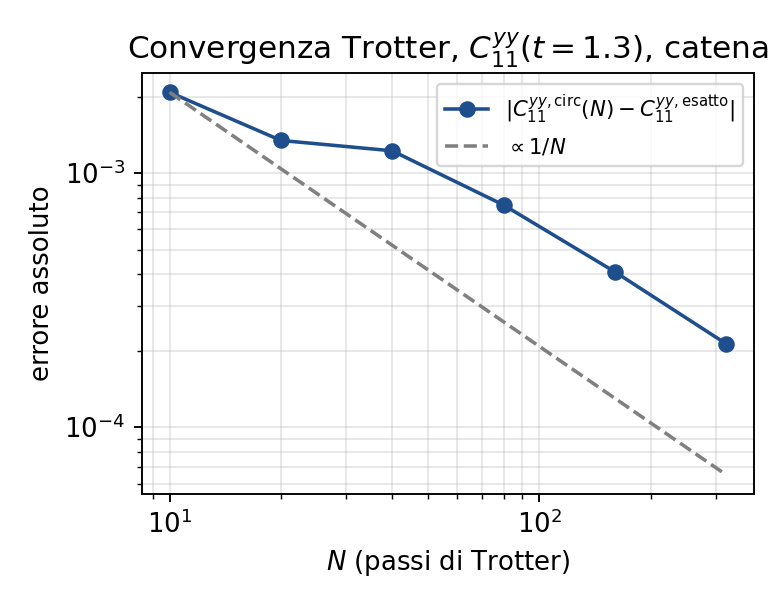
\includegraphics[width=0.55\textwidth]{fig_trotter_trimero_catena.png}
\caption{Errore del circuito rispetto al valore esatto, $C_{11}^{yy}(t{=}1.3)$, in funzione di
$N$. La linea tratteggiata è $1/N$.}
\label{fig:trotter}
\end{figure}

% =====================================================================
\section{La misura}
% =====================================================================

Identica a dimero e anello: due esecuzioni separate ($H$ per Re, $R_x(\pi/2)$ per Im),
$\langle\sigma_z\rangle\simeq(n_0-n_1)/N_\text{shots}$.

\subsection{Validazione a shot finiti: quale errore domina?}

Per $C_{11}^{zz}(t{=}1.3)$ (autocorrelazione ricca), confrontando l'errore di Trotter puro con la
soglia statistica nel caso peggiore:
\begin{center}
\begin{tabular}{lc}
\toprule
Errore di Trotter (statevector vs esatto, $N{=}200$) & $1.07\times10^{-3}$\\
Soglia statistica, caso peggiore ($N_\text{shots}=8192$) & $1.10\times10^{-2}$\\
Rapporto (statistico/Trotter) & $\sim10\times$\\
\bottomrule
\end{tabular}
\end{center}

\begin{ideabox}[Stesso regime dell'anello]
Anche qui l'errore statistico domina, come nell'anello ($\sim16\times$) --- opposto al regime
dimostrativo $R_1$ del dimero. Al punto S0 (Trotter, $D=0.3$) il rapporto è ancora più marcato
($\sim115\times$, misurato su $C_{11}^{zz}$): un punto con $D$ più grande converge più
rapidamente in $N$, spostando ulteriormente il collo di bottiglia sul rumore statistico.
\end{ideabox}

\begin{figure}[htbp]
\centering
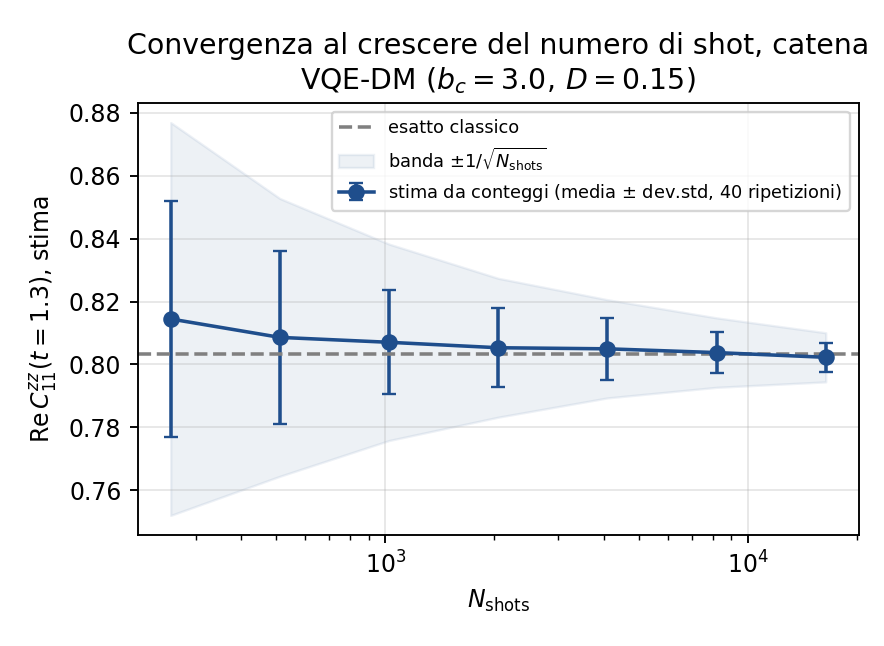
\includegraphics[width=0.62\textwidth]{fig_shot_trimero_catena_vqedm.png}
\caption{Stima di $\mathrm{Re}\,C_{11}^{zz}(t{=}1.3)$ al crescere del numero di shot (media e
dev.\ std.\ su 40 ripetizioni, $N{=}200$). Banda ombreggiata $\pm1/\sqrt{N_\text{shots}}$.}
\label{fig:shotconv}
\end{figure}

% =====================================================================
\section{Il circuito completo e la sua validazione}
\label{sec:validazione}
% =====================================================================

Riferimento classico via esponenziale di matrice diretto (\texttt{scipy.linalg.expm}), non
formula spettrale --- stessa cautela di anello e dimero.

\begin{center}
\begin{tabular}{lcccc}
\toprule
correlatore & $t$ & esatto classico & circuito ($N{=}200$) & $|$residuo$|$\\
\midrule
$C_{11}^{yy}$ & $1.3$ & $+0.3243-0.4919i$ & $+0.3244-0.4922i$ & $3.3\times10^{-4}$\\
$C_{33}^{yy}$ & $1.3$ & $+0.3243-0.4919i$ & $+0.3249-0.4918i$ & $6.3\times10^{-4}$\\
$C_{12}^{yy}$ & $2.7$ & $+0.1069+0.3946i$ & $+0.1111+0.3858i$ & $9.7\times10^{-3}$\\
$C_{11}^{xz}$ & $0.0$ & $0.0000+0.0000i$ & $0.0000-0.0000i$ & $4.6\times10^{-16}$\\
\bottomrule
\end{tabular}
\end{center}

\begin{enumerate}[leftmargin=*]
\item \textbf{Accordo generale} entro l'errore di Trotter atteso.
\item \textbf{Relazione $P_{13}$}, $C_{11}^{yy}=C_{33}^{yy}$: confermata via circuito entro
l'errore di Trotter.
\item \textbf{Zero a $t=0$} ($C_{11}^{xz}$, Cor.\ zero-t0-same): confermato a precisione macchina.
\end{enumerate}

\begin{figure}[htbp]
\centering
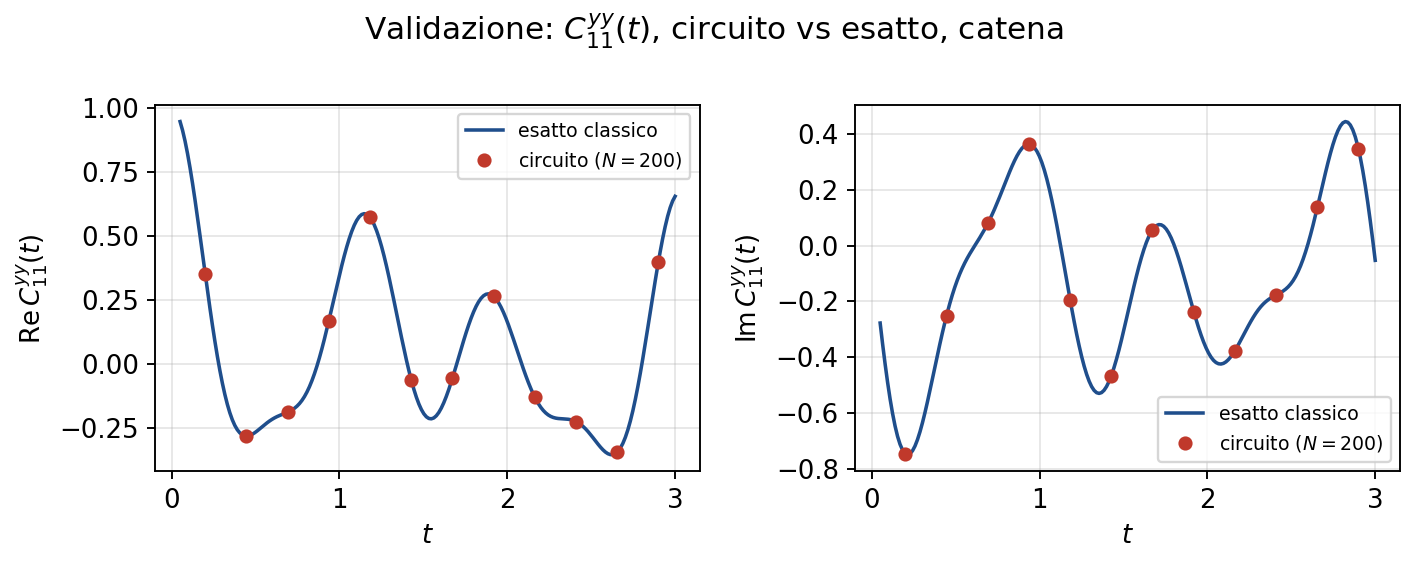
\includegraphics[width=\textwidth]{fig_validazione_trimero_catena.png}
\caption{Validazione continua: $C_{11}^{yy}(t)$, parte reale (sinistra) e immaginaria (destra).
Linea continua: calcolo classico esatto. Punti: circuito quantistico ($N{=}200$). Accordo su
tutto l'intervallo esplorato, per entrambe le componenti.}
\label{fig:validazione}
\end{figure}

\begin{noveltybox}[Verifica mirata: la simmetria potrebbe mascherare un bug di mapping]
Con il ground state (autostato di $P_{13}$), un mapping sito$\leftrightarrow$qubit invertito
sarebbe \textbf{invisibile} a tutti i test precedenti. Verifica dedicata: stato iniziale
\emph{casuale, esplicitamente asimmetrico} sotto $P_{13}$ ($\|P_{13}\psi-\psi\|=1.21$), tutte le
81 combinazioni, $N$ crescente:
\begin{center}
\begin{tabular}{cc}
\toprule
$N$ & errore massimo (81 combinazioni) \\
\midrule
50 & $2.5\times10^{-2}$ \\
200 & $6.3\times10^{-3}$ \\
800 & $1.6\times10^{-3}$ \\
\bottomrule
\end{tabular}
\end{center}
Rapporto $\approx2.0$ raddoppiando $N$ a ogni passo: puro errore di Trotter, nessun bias costante
residuo. Se il mapping fosse invertito l'errore sarebbe $O(1)$ e non scenderebbe con $N$. Mapping
verificato corretto in condizioni che ne avrebbero rivelato l'errore --- non solo sul ground state,
dove sarebbe stato mascherato.
\end{noveltybox}

\subsection{Scan sistematico delle 81 combinazioni, via circuito effettivo}

Mirror di \texttt{scan81\_trimero\_anello.py}: tutte le 81 combinazioni misurate via circuito
(statevector e shot finiti, $8192$ shot), su entrambi i punti di lavoro.

\begin{center}
\begin{tabular}{lcc}
\toprule
& VQE-DM ($D{=}0.15$) & S0 ($D{=}0.3$) \\
\midrule
$|C|$ minimo osservato & $0.1008$ & $0.0168$ \\
errore Trotter, media/max & $1.76\times10^{-3}$ / $3.34\times10^{-3}$ & $1.72\times10^{-3}$ / $3.97\times10^{-3}$\\
errore statistico, media/max & $1.39\times10^{-2}$ / $3.85\times10^{-2}$ & $1.36\times10^{-2}$ / $3.90\times10^{-2}$\\
\bottomrule
\end{tabular}
\end{center}

\paragraph{Nessuno zero, in nessuno dei due punti.} A differenza dell'anello (4 zeri
strutturali confermati esattamente su tutte le 81), qui \textbf{nessuna} delle 81 combinazioni
collassa a zero, in nessuno dei due punti di lavoro --- coerente con $\lambda_\alpha\equiv+1$
(Sez.~\ref{sec:caso2}).

\begin{figure}[htbp]
\centering
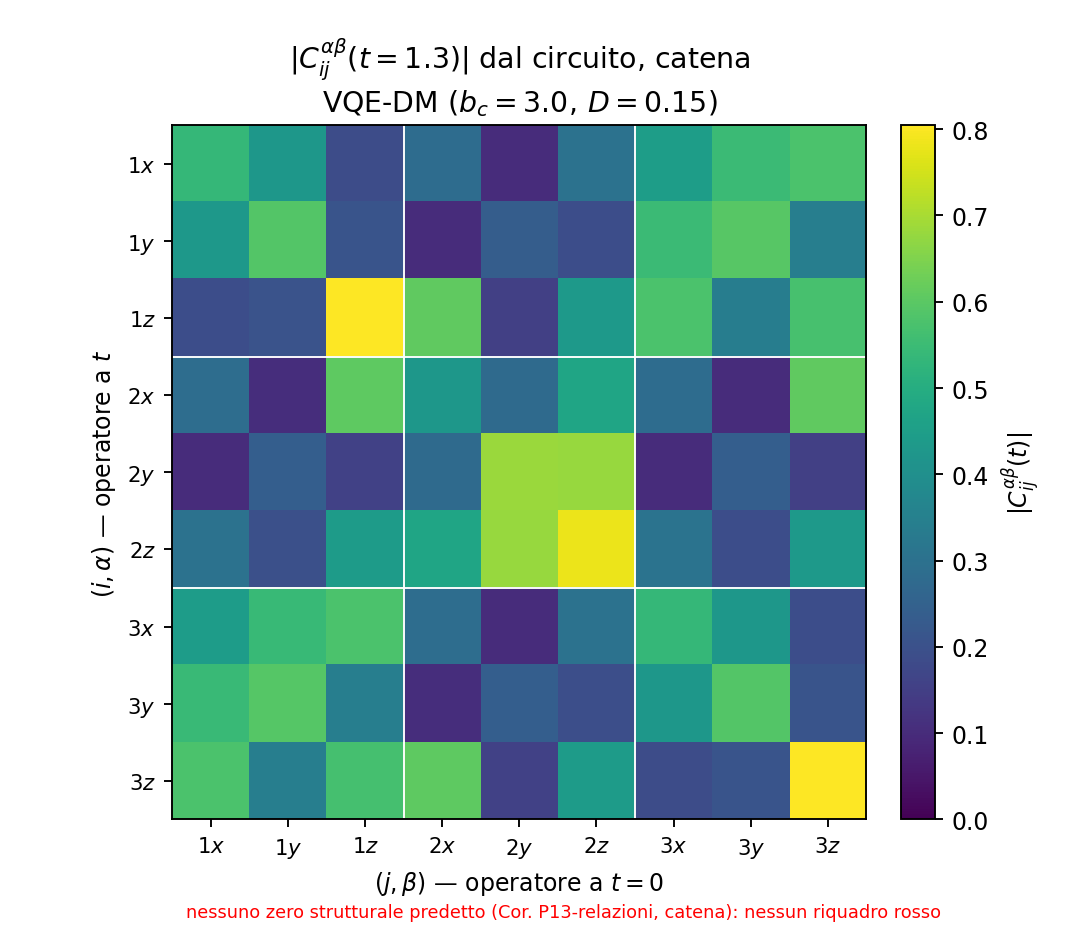
\includegraphics[width=0.72\textwidth]{fig_scan81_trimero_catena_vqedm.png}
\caption{$|C_{ij}^{\alpha\beta}(t{=}1.3)|$, tutte le 81 combinazioni, punto VQE-DM. Nessun
riquadro rosso: nessuno zero strutturale predetto per la catena (a differenza dell'anello).}
\label{fig:scan81}
\end{figure}

% =====================================================================
\section{Riepilogo dei passaggi}
% =====================================================================

\begin{enumerate}[leftmargin=*]
\item $C_{ij}^{\alpha\beta}(t)$, $81$ combinazioni (come l'anello, perché dipende dai siti non
dai legami): complesso, non hermitiano per $t\neq0$, non misurabile direttamente.
\item Ancilla + registro a tre qubit; costruzione dei due rami coerenti identica a dimero e
anello.
\item \textbf{Novità 1 (simmetria, qualitativa)}: il sito fisso (2) della simmetria $P_{13}$
\textbf{non} produce zeri strutturali, a differenza del sito fisso (3) dell'anello --- perché
$\lambda_\alpha\equiv+1$ sempre (nessuna rotazione oltre lo scambio, coerente con l'assenza di
frustrazione nella catena).
\item \textbf{Novità 2 (implementazione)}: $U(t)$ richiede comunque un Trotter a due livelli (due
bond condividono un qubit), come l'anello, ma con la struttura minima (due bond, non tre); in più,
l'opzione \texttt{alternate} (assente nell'anello) cancella il termine chirale di livello 1 al
leading order, con guadagno che dipende criticamente da $D$ e da $N$.
\item Validato su entrambi i punti di lavoro (VQE-DM e S0): accordo entro l'errore di Trotter,
relazione $P_{13}$ confermata via circuito, zero a $t=0$ confermato a precisione macchina, mapping
verificato anche su stato asimmetrico.
\item Scan sistematico delle 81 combinazioni (statevector e shot finiti, entrambi i punti):
nessuno zero in nessuno dei due punti --- coerente con l'assenza di zeri strutturali predetta.
\end{enumerate}

\paragraph{Aperto per il seguito.} Notebook eseguiti (mirror computazionale, già completati);
manuale d'uso e documento di raccolta della fase (in preparazione); rumore di gate reale (Parte 2
della tesi).

\end{document}
